%!TEX root = thesis.tex
\chapter{Evaluation} % (fold)
\label{ch:evaluation}
%- Evaluate the solution and compare existing techniques for personalisation to the ones used in the solution.
This section evaluates the implementation as a solution to the problem of personalising the editorial mix and Constraint Programming as a technology for creating personalised web applications.
%
%\todo[inline]{What things were even better or a little worse than expected regarding the methods you used to solve your problems. How could your project be improved by further work.}

%\subsection{Result}
\section{Test}
The test described in Table~\vref{tab:test-description} was conducted on 7 test persons. This is not a solid ground to base decisions upon, but it has been helpful in finding some tentative problems. Main design choices should, in the further development of this application, be verified on a larger empirical basis.

The editorial mix has been conducted on rules inferred from analysis of conventional newspapers. It has not been verified that the composition of articles using these rules actually satisfies user needs better in a digital environment -- even if users are unaware of them. This could be done by turning constraints on and off in the system and presenting them to users, so they can give their feedback on the best composition. In addition, new rules could be added to test new hypotheses. It could for example be interesting to explore users' preferences on the two rejected reading behaviours presented in \cite{holsanova2006entry}:
\begin{itemize}\itemdist
	\item Readers Prefer new information and expect this to be on the right in the semiotic space
	\item Readers scan the semiotic space before taking a closer look at certain units
\end{itemize}

The next section will evaluate the interface of the application.
%\todo[inline]{NOT ONLY 5 test persons \protect\cite{NielsenTest}. This has been discarded by many.}
%\cite{NielsenTest} says that 5 test persons in a qualitative test is enough to uncover most preferences and issues, but the test included 7 test persons to be more adequate.
%
%\todo[inline]{Hvor langt tid er en artikel interessant > hvor lang tid er en annonce interessant.}

\section{Interface}
In the implemented layout no visual difference between featured articles was supplied. Articles was just supplied with more space if the contents could fill it out. In the further development of the application a distinction between featured and non-featured content should be applied as described in the presented constraints in section~\vref{sec:problem_representation}. This way content distinction can be applied visually.
%\todo[inline]{Implement visual difference between featured articles and non-featured articles.}
%classify items as first and second articles and use layout to distinguish them.

The implemented columns constraints does not always provide good solutions, because they account only for horizontal features of the articles and not vertical. Therefore problems emerge when long-length articles are placed beside short-length articles leaving a lot of white space under the short. The implementation of this fairly complex constraint show that it is possible to implement constraints layout, but that it is hard to formalise and account for every detail. Therefore it worthwhile extracting key features about the layout that is needed to be handled and spend time on reducing constraints to a minimum, let other technologies handle these problems or explore a combination. A constraint that would co-operate with the positioning of articles using jQuery Masonry\sidenote{A layout plugin for jQuery, that arranges elements vertically then horizontally according to a grid.} could be a solution for this. Here it is worth noting that the automatic placement could destroy the combinatorial work of the constraints. However, it seems that jQuery Masonry works to keep the chronological structure of elements, which minimises the harm it can do.
%We follow a strict vertical structure, but there is a lot of work to be done with the horizontal structure

At an early stage, the pagination on a section was discarded, because a preliminary test (ask around) showed that users wanted to scroll down to see the full section. This was also necessary if full-length articles were to be shown, but the reading behaviour analysis suggests that articles should be divided into chunks of subjects, which may be better to visualise using pages. Following the reading behaviours more strictly, the featured article could be shown with large headlines, large images and a longer length excerpt, and stories on the same subject could surround it with only headlines, smaller images and short excerpts. If the user then wants to read one of the articles in full length, he can select it, and the article could be displayed in full, using the whole screen.%Non-featured article he could select it, showing interest in it, and the system could generate a new page where this article is featured. The article should then again be surrounded by new non-featured articles, that of course are not placed anywhere else in the paper.
%
%\todo[inline]{Archive functionality}
%\todo[inline]{Text can be read out loud}
%\todo[inline]{Find more images online}
%\todo[inline]{Negative keywords, using WordNets antonym graph}
%\todo[inline]{Breaking alert, tags på artikler}
%\todo[inline]{har jeg skrevet om at slå constraints fra eller til for at teste?}

Furthermore, \cite{kristin-fredrik.pdf} suggested ads in the application, but it was implemented. It is, however, possible specific to extract keywords and weights for a user on a topic basis. This could be done by direct relevance feedback from the user and by implicit relevance feedback by how long time a user spends on an article, as described in the former chapter. The new weights on keywords can be assigned based on the user behaviour in combination with the calculated weight from the article. This is actually in line with what Google AdSense\sidenote{A program that allows publishers of content sites to serve targeted adverts to site content and audience.} does. AdSense is build on analysing the semantic structure of documents using WordNet, but might include other techniques (\cite{Oingo1} and \cite{Oingo2}).
%\todo[inline]{Give dem de mest optimale ord hele tiden, ville jeg kunne optimere Googles valg af reklamer. Facebook skal key word analysere for at kunne skabe værdi.}
%\todo[inline]{Trending (Google trending): hvad er in for tiden? bruge det til at holde reklamer up-to-date. AdWords eller AdSense?}

The application is implemented with a responsive design, with a layout that is familiar to that of a conventional newspaper. It has explored some possibilities for having full articles in balanced columns with a flat navigational structure of user defined topics.

\section{Content}
This section will analyse and discuss the solution with regards to content.

Similarities were computed with respect to manually defined topics\sidenote{The definitions can be seen in Table~\ref{tab:topic-specification1} and \vref{tab:topic-specification2}.} and with respect to articles in between. To test whether similarities actually make sense it seems logical to look at similarities of articles that match a topic and articles that do not match. The feeds of the gathered articles are often categorised under a certain topic. These topics were saved as tags on each of the articles, and it was then possible to analyse the similarities of articles that hold tags that match the defined topic and which do not. Figure~\ref{fig:sim-analysis} shows averages and minimum and maximum of similarities distributed on the defined topics on articles that hold a tag matching a topic and articles that do not hold a tag matching the topic, respectively.
\begin{figure}[h!tp]
	\myfloatalign
	\subfloat[Similarities of articles that matches the section.\label{fig:sim-match}]{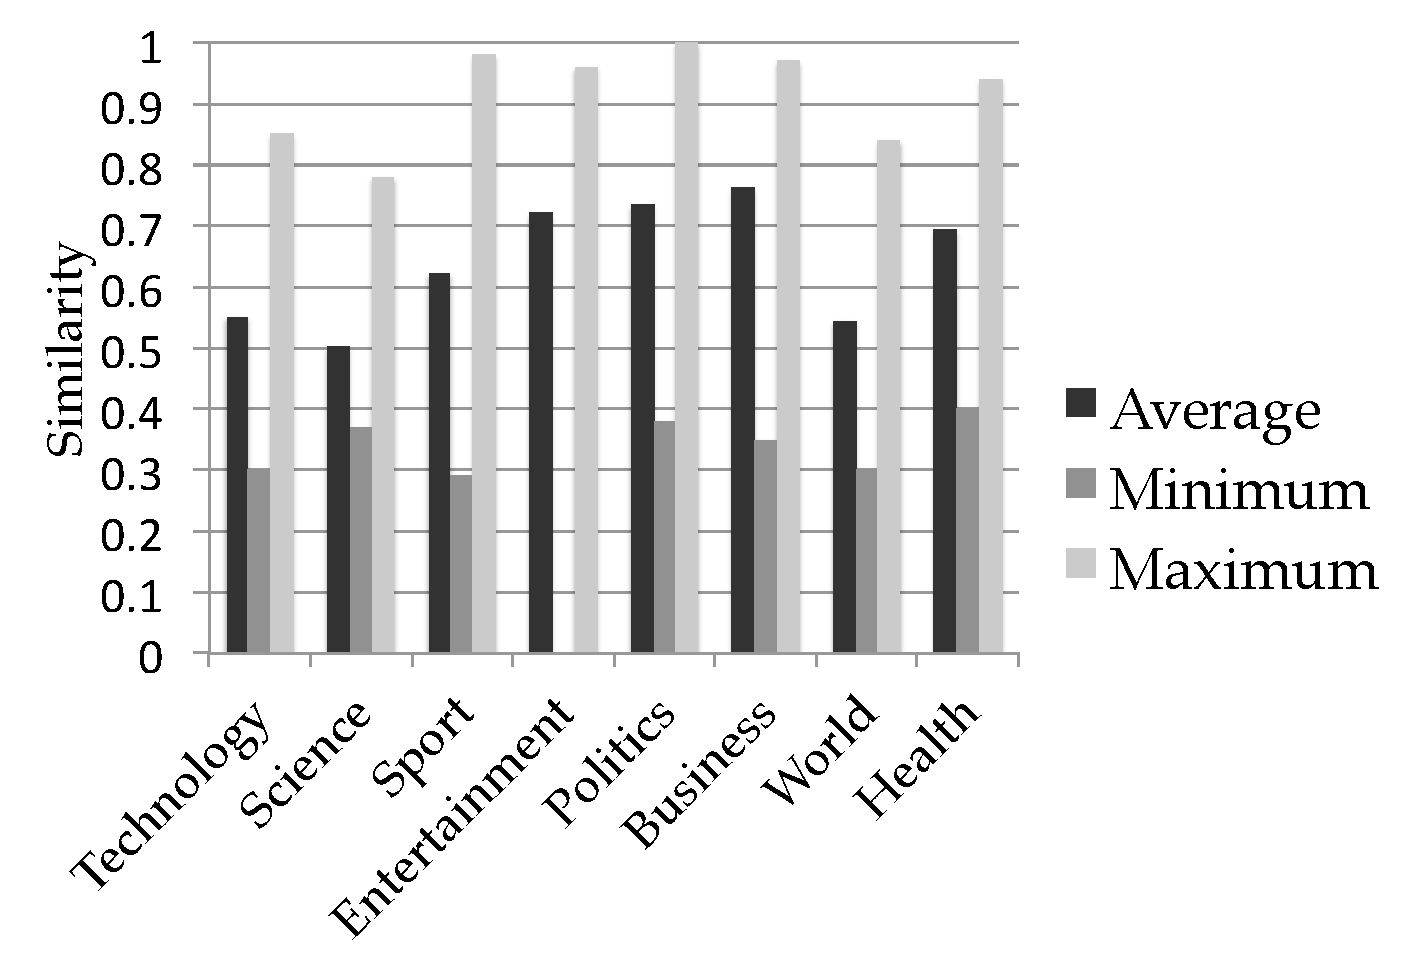
\includegraphics[width=.8\textwidth]{img/sim-max}}%
	\\
	\subfloat[Similarities of articles that do not matches the section.\label{fig:sim-mismatch}]{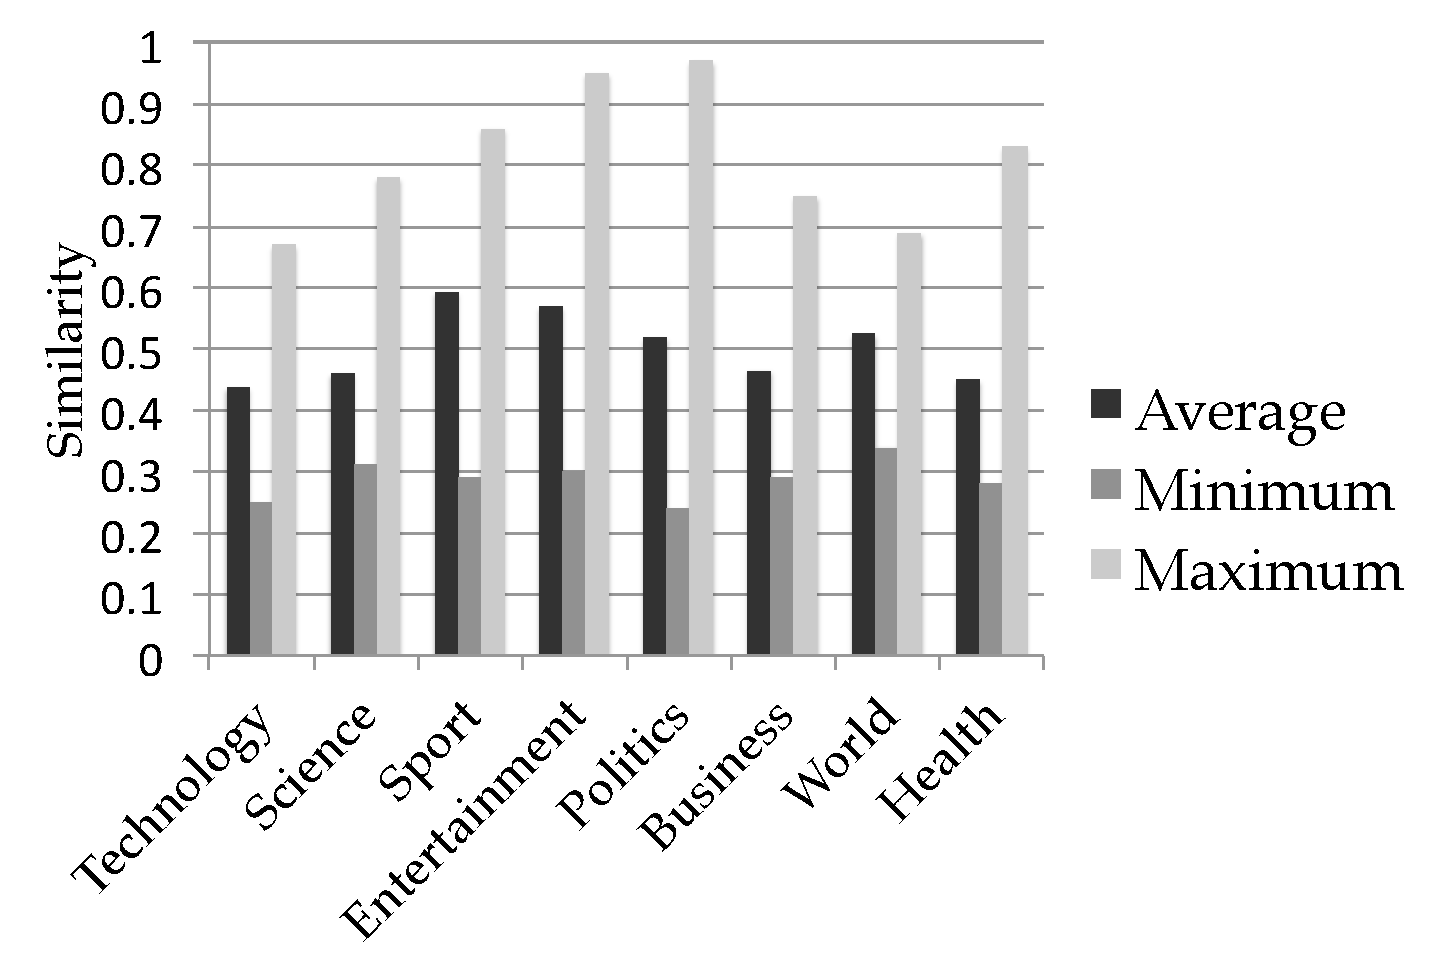
\includegraphics[width=.8\textwidth]{img/sim-min}}%
	%\makebox[\textwidth][l]{
		%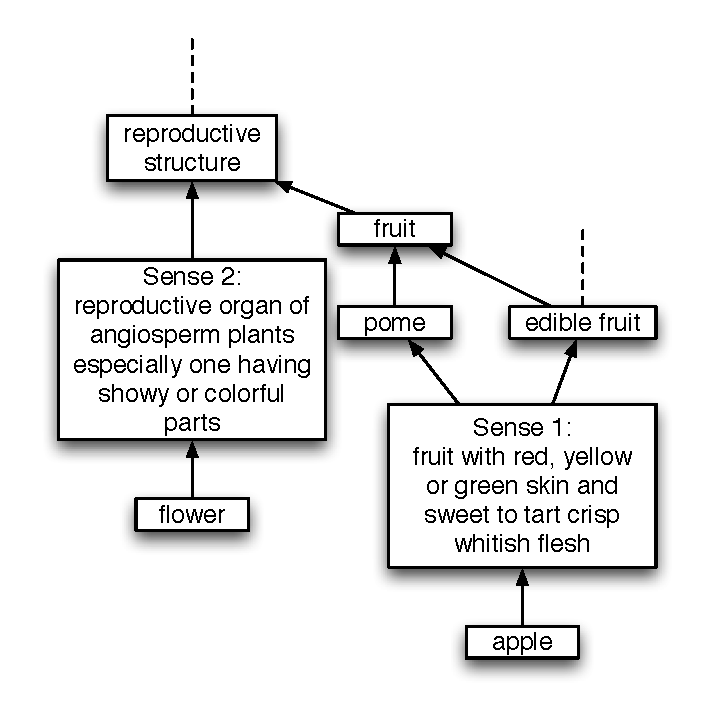
\includegraphics[width=.5\textwidth]{img/flower-apple}
	%}
	%\marginnote{
	%	\begin{minipage}{\marginparwidth}
			\caption{The figure shows respectively matches and mismatches of similarities distributed over sections.}
			\label{fig:sim-analysis}
	%	\end{minipage}
	%}
\end{figure}
The overall average similarities for matching articles is $0.57$ and for mismatching articles it is $0.5$ in a range of $[0;1]$. This seems to be a low match similarity and very high mismatch similarity. The low match similarity could be explained by the definitions of the topics, which might not be the same as what the content providers deem as relevant for these topics. Moreover, the definitions are by no means comprehensive and should more be seen as a subset of their general definitions. The high mismatch similarity average could be explained by the fact that some of the article are actually matches, but are not listed under these topics. An example of this is shown in Figure~\ref{fig:mismatch}.
\begin{figure}[h!tp]
	\myfloatalign
	%\makebox[\textwidth][l]{
		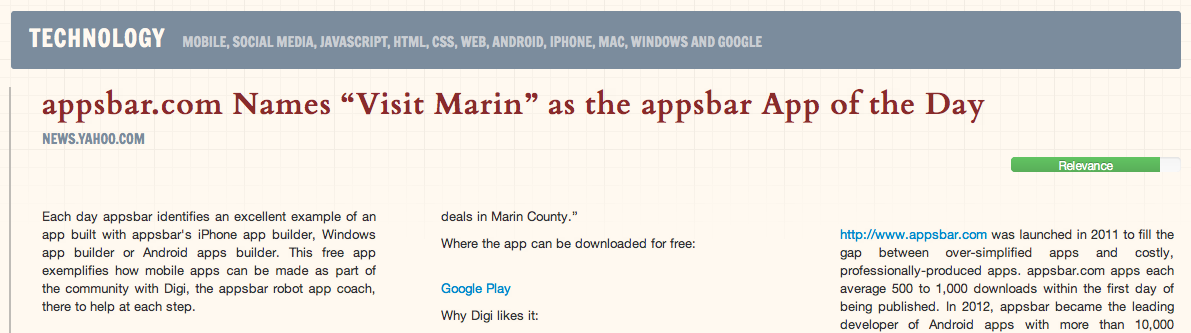
\includegraphics[width=\textwidth]{img/mis-match}
	%}
	\marginnote{
		\begin{minipage}{\marginparwidth}
			\vspace{-120pt}
			\caption{The figure shows an article which has by the system been deemed an article about technology, but is only listed under a business press releases tag by Yahoo.}
			\label{fig:mismatch}
		\end{minipage}
	}
\end{figure}
The fact that most of the used content providers list their feeds under several topics and supplies the articles in all matching feeds could explain this. To handle this, tags were added to the article whenever a URL from the feed was already visited. This did, however, not solve all problems because many content providers listed articles under a different URL for each topic. Looking at the average similarities it is seen that the ``World'' section is near $0.5$ in both matches and mismatches. This could be explained by its definition. It consists mostly proper nouns of parts of the world which are hard to match with proper nouns of countries or cities, that may more often be named in articles.

The similarity between articles is semantically analysed in same way and it is therefore expected to perform equally or better. Better, because the full set of information is available in the article and thereby the analysis has a better chance of extracting keywords, perform enriching and extract entities. It should be noted that the Open Calais API sometimes have problems with extracting entities from a set of keywords instead of sentences, and it could therefore be interesting to explore the possibilities of representing topics based on sentences instead.

In any case, it seems that this analysis is not accurate and a deeper analysis of the similarities in terms of numbers must be done in order to draw any conclusions. However, a qualitative assessment of the results is that the application rarely provides irrelevant articles according to the topics, and that it especially performs well with recognition of entities in articles. And that is even for low similarities. Also, the application seems to be good at following the rules of placing articles that relate near each other, and thereby supplying them in more relevant context than just under the topics, as it is done in conventional newspapers. Finally, some quality of the method can be seen in that the same semantic analysis is done by AdSense and that \cite{116262780379.pdf} has produced promising results with the same algorithm.
%\todo[inline]{Ikke så godt at der ikke har været tid til en ordenlig evaluering... :( Kan ikke lige finde ud af om jeg skal lade være med at skrive det eller hvad.}

It could be interesting to evaluate the precision and recall\sidenote{Precision is the fraction of retrieved instances that are relevant, while recall is the fraction of relevant instances that are retrieved.} points as described in \shortcite{Evaluating-a-User-Model-Based-Personalisation-Architecture-for-Digital-News-Services.pdf}. This could be done by letting a number of test subjects organise a subset of the gathered articles into the given topics and then do an equal analysis as shown in Figure~\ref{fig:mismatch}. Precision and recall evaluation have been done in \cite{Sections-categories-and-keywords-as-interest-specification-tools-for-personalised-news-services.pdf} with categories represented by keywords, it shows poor results for categories of with represented by a few keywords.

In addition, a more comprehensive list of categories and their definitions could also be used. This could either be retrieved by the list of Google News categories\sidenote{\url{http://support.google.com/webmasters/bin/answer.py?hl=en&answer=42993}.} and a WordNet enriched list of key words from Google News list of suggested keywords\sidenote{\url{http://support.google.com/news/publisher/bin/answer.py?hl=en&answer=116037}.} or by the root terms presented in \cite{10-1-1-19-5583}. These can later on be refined by information retrieved by the user behaviour in the system. The user behaviour would also make the system stronger as their relevance feedback can be used to remove false positive and as stated earlier, collaborative filtering to suggest false negatives. The latter could be backed by providing a higher relevance for articles with a subject with many available articles in recent time.
%However, also more advanced techniques of text classification could be used in later stages of the system, like one presented in \shortcite{Evaluating-a-User-Model-Based-Personalisation-Architecture-for-Digital-News-Services.pdf}.
%a Vector Space Model (VSM)
%The paper based on: news items per section, news items per category, maximum number of news items per message required by the user, general relevance of the contents of a given day for a given user, etc. as \cite{Sections-categories-and-keywords-as-interest-specification-tools-for-personalised-news-services.pdf} proposes.
%\cite{Personalizing-your-electronic-newspaper.pdf} suggest virtual communities, or individuals with common interests.

In the application a user could be presented with an article he has seen before. \cite{User-Modeling-for-Adaptive-News-Access.pdf} suggests the nearest neighbour (NN) algorithm approach, using a TF-IDF similarity, to determine whether the story is already known, i.e.\ if the similarity to the NN of articles, that are detected to be already seen, is above a given threshold the article is also determined to be seen. This could be solved by keeping a library of read items and then match new items against this list and down prioritise them if their similarity is too high. However, user might be interested in reading many articles about the same story.
%``Distinguishing between short-term and long-term models has several desirable qualities in domains with temporal characteristics (Chiu and Webb, 1998).'' \cite{User-Modeling-for-Adaptive-News-Access.pdf}.

\cite{Sections-categories-and-keywords-as-interest-specification-tools-for-personalised-news-services.pdf} raise a precision problem in finding relevant news within a single day. This can hopefully be handled by having the user specify in which period of time he wants news and maybe notify the user that solutions might be inaccurate if a limited period of time is chosen, or just provide only articles that are available.
%``just as newspaper must come full of news everyday, regardless of whether anything interesting has happened or not, newspaper sections will carry a certain amount of news independently of their relevance to the section heading, and a personalised news message will feature some news item distantly related to the user profile.''
%Evaluate using the in \shortcite{Evaluating-a-User-Model-Based-Personalisation-Architecture-for-Digital-News-Services.pdf} presented method. Their categorisation based on few keywords (5 as the lowest) to represent a category resulted in poor evaluation, this gives a good motivation for including more keywords and using WordNet to enrich the set of keywords.
%
%\todo[inline]{Maybe find a better example of text classification.}
%
%Use of automatic generation of personal item summaries \cite{fulltext.pdf}

The system does at this point not supply articles of relevance based on the users location. If geo targeting are introduced, using e.g.\ the users IP address or the W3C Geolocation API\sidenote{An effort by the World Wide Web Consortium to standardise an interface to retrieve the geographical location information for a client-side device.}, the system would be able to provide higher relevance according to words that suggest a position on the map. This could also be used to define the ``World'' section even better.
%Use a thesaurus and predefined root terms as in \cite{10-1-1-19-5583} which improves classification; semantic knowledge is more general than keywords.

Furthermore, weights on keywords could be adjusted by a strength (or an uncertainty) of prediction is proposed by \cite{10.1.1.45.5230.pdf}. The uncertainty could be calculated on the basis of how many uses there are of a word, as provided by WordNet.

Finally, some articles presented with the same content over and over again and even contained the main menu of the sites. This was due to some bad results from the scraping using the Readability API. The problem with this is that the menu of news sites often holds keywords that relate to most sections and will therefore be assigned a good relevance to most sections. Because of this, these articles will show up more regularly than others, which disturbs the results from the compositions. Moreover, it could also explain some of the causes to the high relevance mismatch mean derived from the similarity analysis earlier. The problem could be solved with a better sanitising of HTML and standardising of the content. This would remove odd looking elements.

\section{Functionality}
In order to come closer to understanding what conventional newspapers does in terms of editorial rules, it could be interesting to analyse their component structure, e.g.\ using the algorithm presented in \cite{00953970.pdf}. It could also be interesting to establish a co-operation with newspaper editors to extract rules.
%Noget om hvordan programmet samler keywords med vægte for en bruger?
%\todo[inline]{Count the number of sources have included an articles that are very similar to find the breaking factor. Har jeg ikke skrevet det her?}

%$O(n+10 \cdot n(c + c \cdot v + 40n \cdot c \cdot v) )$
The asymptotic running time of the algorithm is $O(m+n^2cv)$, where $m$ is number of articles provided to solve the problem with, $n$ is number of variables in the problem, $c$ is the number of constraints and $v$ is the number of variables a constraint is defined on. This means that the running time is very much dependent on the problem definition, but also of the number of articles given. The function is actually only provided with a subset of the full library based on relevance to spare computation time, but the upper bound remains because it potentially could provide the full library, whereas in practise only a certain percentage constitutes the articles used. More crucially, the running time is polynomially dependent on the number of articles need in the section multiplied by the constraints and the number of variables a constraint is defined on. It is a high running time, but many actions can be taken towards optimising the algorithm, e.g.\ the use of local search techniques, like hill climbing and simulated annealing. Also, the very effective constraint propagation has not been implement, which can aid the algorithm in removing values that are inconsistent with the problem. However, the algorithm is guided to solve the problem both by the MCV heuristic and by the violations of the constraints. Moreover, it is possible to decompose and organise the constraints to aid the algorithm in solving the problem.
%\todo[inline]{hard constraints are not implemented. Should I mention this??}
%Model-View-Control using backbone.js
%Paging: single page web apps + manipulation the browser history \url{https://developer.mozilla.org/en/DOM/Manipulating_the_browser_history}

Furthermore, the CPL only works on finite domains and propagating through many values causes many iterations. Instead it could be interesting to explore a combination of values and ranges in domains. A range could be defined by a start value, a step size and an end value, e.g.\ the list $[0,2,4,6,8,10]$ would be represented by $[0;1]$ with step size $0.2$. This way a whole range could be discarded in a propagation step by looking at its maximum and minimum value. Moreover, if the range holds a potential valid value it can be divided into smaller ranges and their minimum and maximum values may be examined. This divide-and-conquer technique may continue until the search reaches atomic values, which is determined by the step size of the range. If some atomic values and ranges seems to fulfil the constraints they should be kept in the domain.

Moreover, as an answer to the stated hypothesis in section~\vref{sec:hypothesis}, it was possible to personalise the editorial mix and solve the problem with CP and new rules can easily be added or existing ones can be changed. A by-product of the implementation was even a general purpose solver for combinatorial personalisation problems. The library may even be used for other purposes, as long as the problems can be modelled by means of values, variables, domains and constraints. This means that CP was indeed applicable to personalisation problems. The library should, furthermore, be understandable for developers to use it, even if they do not have insight in CP. Finally, it is prepared for implementation of constraint propagation and an automatic ordering of constraints, to optimise the running time for the solver.

% section evaluation (end)